\scanpage{54}\mspage{12}
\deleted{distincte \unsure{des|de} \unsure{$\notin$|$\varnothing$|$\ell$}} $\in I\setminus J$, de façon que les trois
$D_{a_i}$ soient non concourantes, on exige
$(1^\circ)$ que l'\deleted{configuration}\inserted{arr.\ 1-dim} $K_{J'}$ de 6 droites obtenu
soit du cas (\deleted{\unsure{II}}I) ou (II) ci dessus, et
$(2^\circ)$ que l'orientation de $K_J$ défini par la
prescription précédente ne dépende pas du
choix de $J'$.

Il reste enfin à regarder le cas où
quel que soit le système $a_i$ $D_{a_i}$ ($D_{a_i}\in I\setminus J$
passant par $a_i$), celles-ci sont concourantes.
% slanted
\margin{\unsure{de plus au|de plus aucun} fait que $D_{j\in I\setminus J}$ \unsure{passe} par un des trois sommets}
Mais cela implique que \deleted{l'arrang\textsuperscript{t} est} $\operatorname{card} I=6$,
et que l'arrang\textsuperscript{t} est \inserted{isomorphe à} l'arrangement
\unsure{standart|standard} \deleted{de} formé de $7=4+3$ sommets
et 6 ps. droites (qui sont des triangles),
\figure{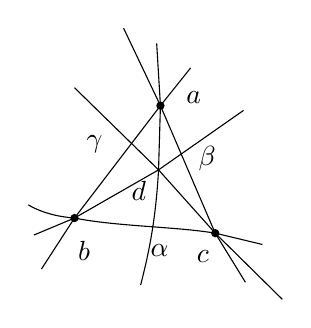
\begin{tikzpicture}[x=.012cm,y=-.012cm]
\draw (29,293)--(64,239)--(155,120)--(187,80);
\draw (116,38)--(155,120)--(213,255)--(245,307);
\draw (151,54)--(155,120)--(153,188).. controls (150,241) and (143,275)..(134,310);
\draw (64,101)--(153,188)--(213,255)--(284,325);
\draw (15,225).. controls (32,235) and (51,238)..(64,239).. controls (109,248) and (171,248)..(213,255)--(263,267);
\draw (21,257)--(64,239)--(153,188)--(243,125);
\fill (155,120) circle (1.5pt); \fill (64,239) circle (1.5pt); \fill (213,255) circle (1.5pt);
\node[right] at (172,111) {$a$}; \node[below] at (74,253) {$b$}; \node[below] at (200,263) {$c$};
\node[below left] at (150,190) {$d$}; \node[below] at (154,257) {$\alpha$};
\node[right] at (185,176) {$\beta$}; \node[left] at (104,161) {$\gamma$};
\end{tikzpicture}}
avec quatre sommets triples, les six ps.
droites étant les ps. droites qui les relient
deux à deux, les trois points d'intersection
supplémentaires étant les intersection des
paires de ps. droites ``opposées''. La situation
combinatoire 1-dimensionnelle (ne comport\textsuperscript{t}
que des triangles) est entièr\textsuperscript{t} décrite
par l'ens des quatre sommets triples.
La situation 2-dimensionnelle correspondante
est aussi \unsure{standart|standard} ($=$ groupe d'autom $\unsure{\mathfrak S|\mathscr S}_4$)
On trouvera la description suivante :
% archive sheet number: 53
